%!TEX root=finmath1.tex
\stopchaptertoc

\part{Дополнения к лекциям}
\titleformat{\chapter}[display]{\bfseries\Large}{\underline{Дополнение~\thechapter}}{0.5em}{}
\titlecontents{chapter}[0em]{}{\textbf{Дополнение\ \thecontentslabel.}\hspace{2mm}}{}{\dotfill\contentspage}
\setcounter{chapter}{0}
\renewcommand{\theHchapter}{A\arabic{chapter}}%

% \begingroup
% \renewcommand{\clearpage}{}
% \phantomsection
% \addcontentsline{toc}{chapter}{\textbf{Приложения}}
% \begin{center}
% \Large\bf \rule[1.5mm]{1cm}{1pt}\quad \textsc{Приложения}\quad \rule[1.5mm]{1cm}{1pt}
% \end{center}

\chapter{Предел модели \crr}
\label{ch:crr-limit}

Здесь мы покажем, что если перейти к пределу в модели \crr\ при <<частоте торговли>>, стремящейся к бесконечности, то получится модель \bs.
В частности, отсюда можно получить формулу \bs\ для цен европейских опционов колл и пут.
%\endgroup

\section{Предел цен рискового и безрискового активов}

Рассмотрим серию моделей \crr, индексированных параметром $n$, в которых время изменяется дискретно по шагам $t=0,1,\dots,Tn$, а параметры изменения цен активов имеют вид
\[
u_n = \frac{\sigma}{\sqrt n}, \qquad d_n = -\frac{\sigma}{\sqrt n}, \qquad r_n = \frac{r}{n},
\]
где величины $\sigma>0$, $r\in \R$ и $T\in\mathbb{N}$ фиксированы, а $n\to\infty$. Начальное значение цены рискового актива $S_0>0$ считается одинаковым во всех моделях. 
Будем предполагать, что рассматриваются достаточно большие $n$, так что выполнено условие безарбитражности $d_n < r_n < u_n$.
Нормирующие коэффициенты $1/\sqrt{n}$ и $1/n$ в формулах для $u_n,d_n$ и $r_n$ специально подобраны так, чтобы получился нетривиальный предел.

Рассматриваемую ситуацию можно представлять себе таким образом, что за единицу календарного времени (например, день, месяц, или год) разрешается торговать $n$ раз.
Тогда в промежутке календарного времени длины $T$ единиц поместится $Tn$ шагов модели \crr. 

Пусть $B^{(n)}_t$, $S^{(n)}_t$, $t=0,\dots,Tn$, обозначают цены безрискового и рискового активов в модели с индексом $n$.
Мы приведем два результата о сходимости цен при $n\to\infty$.
Их отличие будет в том, что первый результат дает сходимость только для фиксированного $T$, а второй результат содержит более сильное утверждение о сходимости траекторий.
Первый результат мы докажем полностью, а во втором лишь сошлемся на известную предельную теорему для случайных блужданий.

Далее пусть $\Q^{(n)}$ обозначает риск-нейтральную вероятность в модели $n$.

\begin{proposition}
\label{crrl:p:convergence-1}
Для любого фиксированного $t\in\mathbb{N}$ и $n\to\infty$ имеет место сходимость
\begin{align}
\label{crrl:b-limit}
&B_{tn}^{(n)} \to e^{rt},\\
\label{crrl:s-limit}
&S_{tn}^{(n)} \xrightarrow{\text{d}} S_0 \exp\biggl(\Bigl(r- \frac{\sigma^2}{2}\Bigr) t + \sigma W_t\biggr),
\end{align}
где $W_t$ "--- нормальная случайная величина с нулевым средним и дисперсией $t$. 
Предел \eqref{crrl:b-limit} понимается в смысле сходимости числовой последовательности, а предел \eqref{crrl:s-limit} в смысле сходимости случайных величин по распределению, где распределение $S_{tn}^{(n)}$ берется относительно риск-нейтральной вероятности $\Q^{(n)}$.
\end{proposition}

\begin{proof}[Доказательство]
Сходимость \eqref{crrl:b-limit} следует из <<первого замечательного предела>>:
\[
B^{(n)}_{tn} = (1+r_n)^{tn} = \biggl(1 + \frac rn\biggr)^{tn} \to e^{rt}.
\]

Чтобы доказать второе утверждение, представим цену рискового актива в виде $S^{(n)}_{tn} = S_0\exp( a_n \xi_{tn} + b_n tn)$,
где $\xi_{tn}$ имеет биномиальное распределение с параметрами $(tn, q_n)$, и
\[
a_n = \ln \Bigl(1 + \frac{\sigma}{\sqrt n}\Bigr) 
  - \ln\Bigl(1 - \frac\sigma{\sqrt n}\Bigr), \quad
b_n = \ln \Bigl(1-\frac{\sigma}{\sqrt n}\Bigr),\quad 
q_n = \frac{r_n-d_n}{u_n-d_n}.
\]
Показатель экспоненты в формуле для $S_{tn}^{(n)}$ можно переписать в виде
\[
\begin{split}
a_n\zeta_{tn} + b_ntn &= a_n\sqrt{tnq_n(1-q_n)}\cdot \frac{\zeta_{tn} - q_n tn}{\sqrt{ tnq_n(1-q_n)}} + (a_nq_n +b_n)tn \\
&:= A_n\cdot B_n + C_n.
\end{split}
\]
Раскладывая по формуле Тейлора, находим
\[
a_n = \frac{2\sigma}{\sqrt n} + o\Bigl(\frac1n\Bigr), \qquad
b_n = -\frac{\sigma}{\sqrt n} - \frac{\sigma^2}{2n}+ o\Bigl(\frac1n\Bigr),\qquad
q_n = \frac 12 + \frac{r}{2\sigma\sqrt n}+ o\Bigl(\frac1n\Bigr).
\]
Отсюда нетрудно найти пределы неслучайных последовательностей $A_n$ и $C_n$: имеем $A_n \to \sigma \sqrt t$ и $C_n \to \Bigl(r - \frac{\sigma^2}{2}\Bigr)t$.
Кроме того, согласно центральной предельной теореме, $B_n \to N(0,1)$ по распределению.
Подставляя полученные пределы в формулу для $S_{tn}^{(n)}$, получаем доказываемое утверждение.
\end{proof}

Чтобы сформулировать второе предложение, построим кусочно"=постоянное вложение\footnote{Результат останется справедливым, если рассматривать кусочно--линейное вложение.} рассматриваемых дискретных моделей в непрерывное время, определив неслучайную функцию $\hat B_t^{(n)} = B_{[tn]}^{(n)}$ и случайный процесс $\hat S_t^{(n)} = S_{[tn]}^{(n)}$, где $t\in[0,T]$. Рис.~\ref{crrl:fig} качественно показывает, как выглядит процесс $\hat S_t^{(n)}$.

\begin{figure}[h]
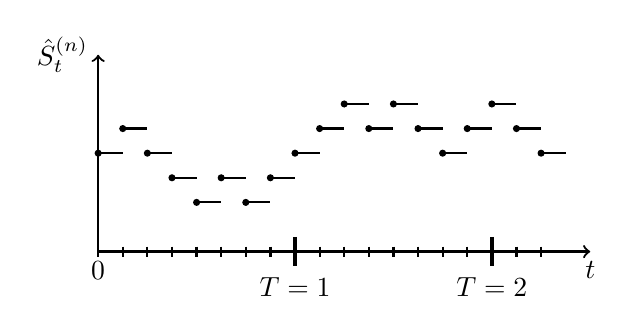
\begin{tikzpicture}[scale=1.25]
\draw[thick,->] (0,0) node[below] {$0$} 
  -- (5,0) node[below] {$t$};
\draw[thick,->] (0,0) -- (0,2) node[left] {$\hat S^{(n)}_t$};
\draw[thick] (0,1) --  (0.25,1);
\draw[thick] (0.25,1.25) -- (0.5,1.25);
\draw[thick] (0.5,1) -- (0.75,1);
\draw[thick] (0.75,0.75) -- (1,0.75);
\draw[thick] (1,0.5) -- (1.25,0.5);
\draw[thick] (1.25, 0.75) -- (1.5, 0.75);
\draw[thick] (1.5,0.5) -- (1.75,0.5);
\draw[thick] (1.75,0.75) -- (2,0.75);
\draw[thick] (2,1) -- (2.25,1);
\draw[thick] (2.25,1.25) -- (2.5,1.25);
\draw[thick] (2.5,1.5) -- (2.75,1.5);
\draw[thick] (2.75, 1.25) -- (3,1.25);
\draw[thick] (3,1.5) -- (3.25,1.5);
\draw[thick] (3.25,1.25) -- (3.5,1.25);
\draw[thick] (3.5,1) -- (3.75,1);
\draw[thick] (3.75,1.25) -- (4,1.25);
\draw[thick] (4,1.5) -- (4.25,1.5);
\draw[thick] (4.25,1.25) -- (4.5,1.25);
\draw[thick] (4.5,1) -- (4.75,1);
\filldraw (0,1) circle (0.03); 
\filldraw (0.25,1.25) circle (0.03);
\filldraw (0.5,1) circle (0.03);
\filldraw (0.75,0.75) circle (0.03);
\filldraw (1,0.5) circle (0.03);
\filldraw (1.25,0.75) circle (0.03);
\filldraw (1.5,0.5) circle (0.03);
\filldraw (1.75,0.75) circle (0.03);
\filldraw (2,1) circle (0.03);
\filldraw (2.25,1.25) circle (0.03);
\filldraw (2.5,1.5) circle (0.03);
\filldraw (2.75,1.25) circle (0.03);
\filldraw (3,1.5) circle (0.03);
\filldraw (3.25,1.25) circle (0.03);
\filldraw (3.5,1) circle (0.03);
\filldraw (3.75,1.25) circle (0.03);
\filldraw (4,1.5) circle (0.03);
\filldraw (4.25,1.25) circle (0.03);
\filldraw (4.5,1) circle (0.03);
\draw[very thick] (2,0.15)--(2,-0.15) node[below,black] {$T=1$};
\draw[very thick] (4,0.15)--(4,-0.15) node[below,black] {$T=2$};
\foreach \i in {0,0.25,0.5,0.75,1,1.25,1.5,1.75,2.25,2.5,2.75,3,3.25,3.5,3.75,4.25,4.5} 
\draw[thick] (\i,0.05)--(\i,-0.05);
\end{tikzpicture}
\centering
\caption{Качественный вид процесса $\hat S_t^{(n)}$.}
\label{crrl:fig}
\end{figure}

Далее под сходимостью случайных процессов по распределению будем понимать сходимость порождаемых ими мер на пространстве Скорохода.
Подробнее о сходимости случайных процессов, см., например, \cite{BulinskiShiryaev04}, гл.~V. 
О броуновском движении и геометрическом броуновском движении, которые упоминаются в предложении, см.~лекцию \ref{ch:processes}.

\begin{proposition}
Функции $\hat B^{(n)}$ сходятся равномерно по $t\in[0,T]$: $\hat B^{(n)}_t \rightrightarrows e^{rt}$ при $n\to\infty$.
Процессы $\hat S^{(n)}$ сходятся по распределению: $(\hat S_t^{(n)})_{t\in[0,T]} \xrightarrow{\text{d}} (\hat S_t)_{t\in[0,T]}$, где предельный процесс имеет вид $\hat S_t = S_0 \exp((r- \frac{\sigma^2}{2}) t + \sigma W_t)$ со стандартным броуновским движением $W$, и, таким образом, $\hat S$ является геометрическим броуновским движением.
\end{proposition}

Доказательство утверждения для $\hat B^{(n)}$ остается в качестве упражнения, а доказательство для $\hat S^{(n)}$ является следствием принципа инвариантности Донскера"--~Прохорова (см.~\cite{BulinskiShiryaev04}, гл.~V).


\section{Предел цен платежных обязательств}

\begin{proposition}
\label{crrl:p:convergence-2}
Пусть $f(s)$ является непрерывной неотрицательной функцией на $\R_+$, удовлетворяющей условию $f(s) \le c(1+s^p)$ для всех $s\ge 0$, где $c$ и $p$ "--- некоторые неотрицательные константы.
Обозначим за $V^n$ цену (в момент времени 0)  платежного обязательства с выплатой $f(S_{Tn}^{(n)})$, производимой в момент времени $Tn$ в модели с индексом $n$.
Тогда 
\begin{equation}
\label{crrl:limit}
V^n \to e^{-rT} \E f(S_T)\ \text{при}\ n\to\infty,
\end{equation}
где $S_T = S_0 \exp((r-\frac{\sigma^2}{2})T + \sigma W_T)$, а величина $W_T$ имеет нормальное распределение с нулевым средним и дисперсией $T$.
\end{proposition}

\begin{remark}
В правой части формулы \eqref{crrl:limit} стоит ничто иное, как цена платежного обязательства с функцией выплаты $f$ в модели \bs.
В частности, отсюда получается формулу \bs\ для цен европейских опционов колл и пут, если вычислить математическое ожидание.
\end{remark}

\begin{proof}[Доказательство предложения \ref{crrl:p:convergence-2}]
Заметим, что $V^n = \E^{Q^{(n)}} f(S_{Tn}^{(n)}) / B_{Tn}^{(n)}$. 
Как показано в предложении \ref{crrl:p:convergence-1}, имеем $B_{Tn}^{(n)} \to e^{rT}$, а также $S_{Tn}^{(n)} \xrightarrow{\text{d}} S_T$.
Тогда, если функция $f$ ограничена, то доказываемое утверждение следует из определения сходимости по распределению%
\footnote{Сходятся математические ожидания любой непрерывной ограниченной функции от рассматриваемой последовательности случайных величин (одно из эквивалентных определений сходимости по распределению).}.

Чтобы доказать утверждение для неограниченной функции $f$, нам потребуются следующие вспомогательные результаты.

\begin{definition}
Последовательность случайных величин $Y_n$ называется \emph{асимптотически равномерно интегрируемой}, если 
\[
\lim_{n\to\infty} \limsup_{m\to\infty} \E|Y_n| \I(|Y_n|>m) = 0.
\]
\end{definition}

\begin{lemma}[см.~\cite{VanDerVaart98}, теорема 2.20]
\label{crrl:l:aui}
Пусть $f(x)$ "--- непрерывная функция на $\R$, а последовательность случайных величин $X_n$ сходится к $X$ по распределению, причем последовательность $f(X_n)$ асимптотически равномерно интегрируема.
Тогда $\E f(X_n) \to \E f(X)$. 
\end{lemma}

Вернемся к доказательству предложения \ref{crrl:p:convergence-2}. Возьмем случайные величины $X_n$ с таким же распределением, как у $S_{Tn}^{(n)}$ по мере $\Q^{(n)}$, а $X$ с таким же распределением, как у $S_T$.
Покажем, что последовательность $Y_n = f(X_n)$ асимптотически равномерно интегрируема.  

Используя неравенства Коши"--~Буняковского и Чебышева, получаем оценку
\begin{equation}
\label{crrl:bound}
\E|Y_n| \I(|Y_n|>m) \le \sqrt{\E Y_n^2} \P(|Y_n| > m) \le \sqrt{\E Y_n^2} \frac{\E Y_n^2}{m^2} = \frac{(\E Y_n^2)^{\frac32}}{m^2}.
\end{equation}
Из условия $f(s) \le c(1+s^p)$ получаем
\[
\E Y_n^2 \le  c^2 + 2c\E X_n^p + c^2\E X_n^{2p}.
\]
Заметим, что $\E X_n^p = S_0^p ((1+u_n)^p q_n + (1-u_n)^p(1-q_n))^{Tn}$, и, используя формулу Тейлора можно непосредственно проверить, что $\E X_n^p$ имеет конечный предел при $n\to \infty$.
Следовательно, найдется константа $c_1$ такая, что $\E X_n^p < c_1$ при всех $n$.
Аналогично, $\E X_n^{2p} < c_2$ при всех $n$, и тогда $\E Y_n^2 \le c_3$ для некоторой константы $c_3$.
Отсюда и из оценки \eqref{crrl:bound} следует асимптотическая равномерная интегрируемость последовательности $Y_n$.
Применяя лемму \ref{crrl:l:aui}, доказательство теперь можно завершить так же, как в случае ограниченной функции $f$. 
\end{proof}
